\secrel{1. Introduction to Practical Electronics\\\ru{Введение в практическую
электронику}}\secdown

\clearpage\section*{\ru{От переводчика}}
\addcontentsline{toc}{section}{\ru{От переводчика}}

Эта часть основана на переводе книги:
\bigskip

\textbf{An Introduction to Practical Electronics, Microcontrollers and Software
Design}

Second Edition, 01 May-2014

\copyright\ Bill Collis

\url{www.techideas.co.nz}

\bigskip
Мы признательны автору за разрешение использовать материалы его книги в
русскоязычном варианте <<Азбуки>>, и конечно он вполне заслуженно включен в
основные соавторы этой книги.

\bigskip
We are grateful to the author for permission to use materials of his book in the
russian version of <<Azbuka>>, and of course he was deservedly included in the
main co-authors of this book.

\bigskip
\begin{verbatim}
From: Bill Collis <Bill.Collis@..........nz>
Date: 2014-11-24 0:53 GMT+04:00
Subject: Electronis Book
To: "dponyatov@gmail.com" <dponyatov@gmail.com>

Hi Dmitry
thanks for your email.
I am looking at the future of the book myself and thinking I will open source
it. If you will only be in using it in Russian language then that is ok and you
need to reference the original book.

Thanks
Bill
\end{verbatim}


This book has a number of focus areas.

\ru{Эта книга \copyright\note{оригинал: \cite{bcollis}\ B.Collis The
Introduction to Practical Electronics\ldots}\ имеет следующий ряд основных
направлений:}

\begin{itemize}
  \item Electronic component recognition and correct handling
\\\ru{Распознавание электронных компонентов и их правильное использование}
  \item  Developing a solid set of conceptual understandings in basic
  electronics.
\\\ru{Наработка цельного набора компетенций по основам электроники}
  \item  Electronic breadboard use
\\\ru{Использование макетных плат}
  \item  Hand soldering skills
\\\ru{Навыки ручной пайки}
  \item  Use of Ohm's law for current limiting resistors
\\\ru{Использование закона Ома для выбора токоограничивающих резисторов}
  \item  The voltage divider
\\\ru{Делитель напряжения}
  \item  CAD PCB design and manufacture
\\\ru{Использование EDA CAD\note{[E]lectronic [D]esign [A]utomation, САПР
автоматизации проектирования электроники}\ для разработки и подготовки
производства печатных плат}
  \item  Microcontroller programming and interfacing
\\\ru{Программирование микроконтроллеров и их сопряжение с внешними
устройствами}
  \item  The transistor as a switch
\\\ru{Использование транзистора в режиме ключа}
  \item  Power supply theory
\\\ru{Теория источников питания}
  \item  Motor driving principles and circuits
\\\ru{Принципы и схемы электропривода}
  \item  Modelling solutions through testing and trialing
\\\ru{Навыки отладки схем, их тестирования и испытаний}
  \item  Following codes of practice
\\\ru{Следование принципам обучения через практику}
  \item  Safe workshop practices
\\\ru{Безопасные приемы работы}
\end{itemize}

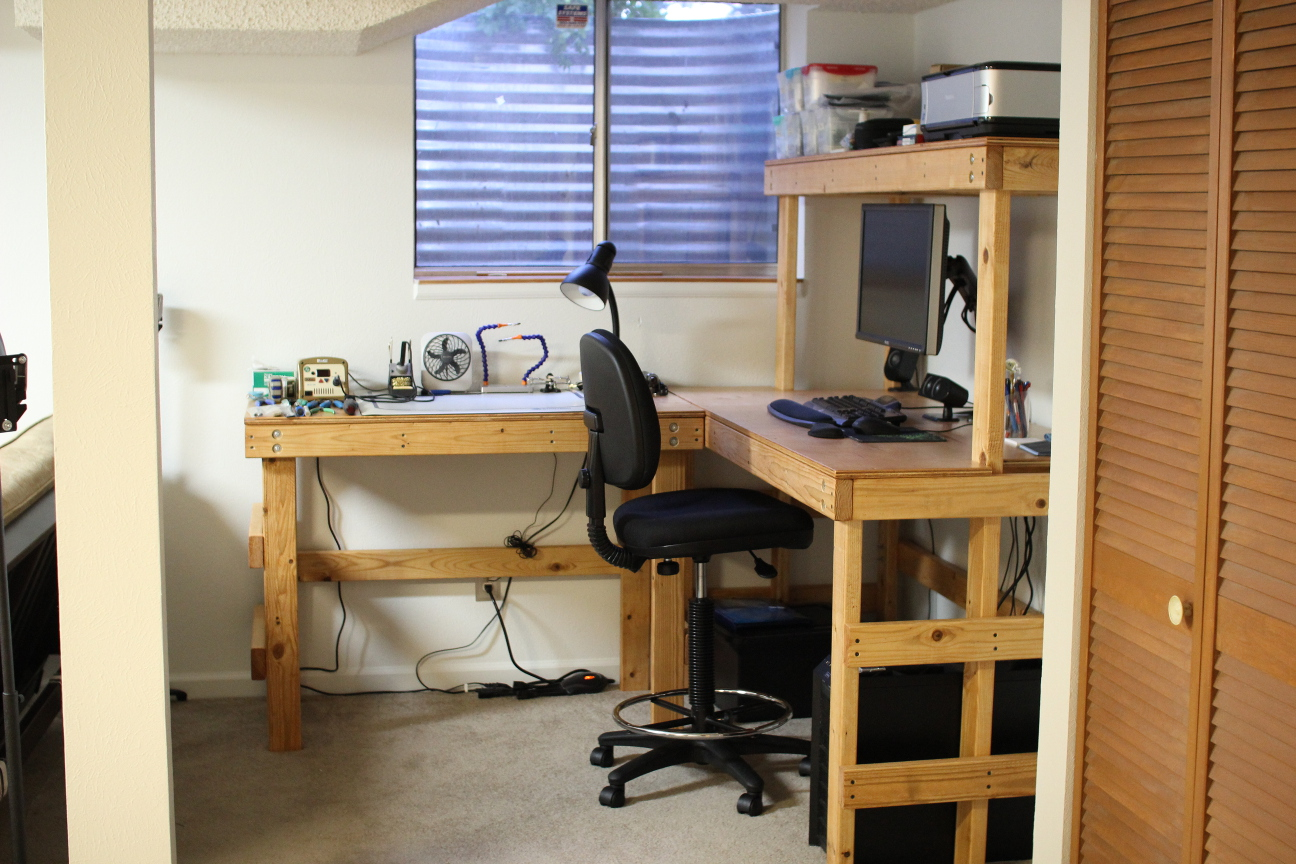
\includegraphics[height=0.33\textheight]{bcollis/1wbench.jpeg}
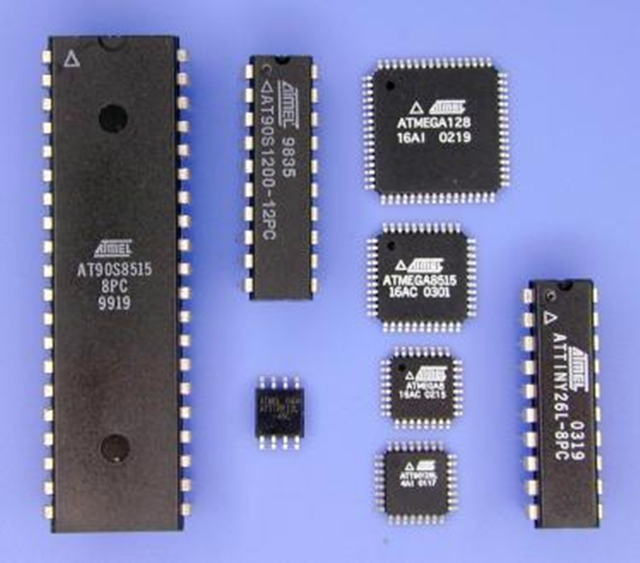
\includegraphics[height=0.33\textheight]{bcollis/1atmels.jpeg}
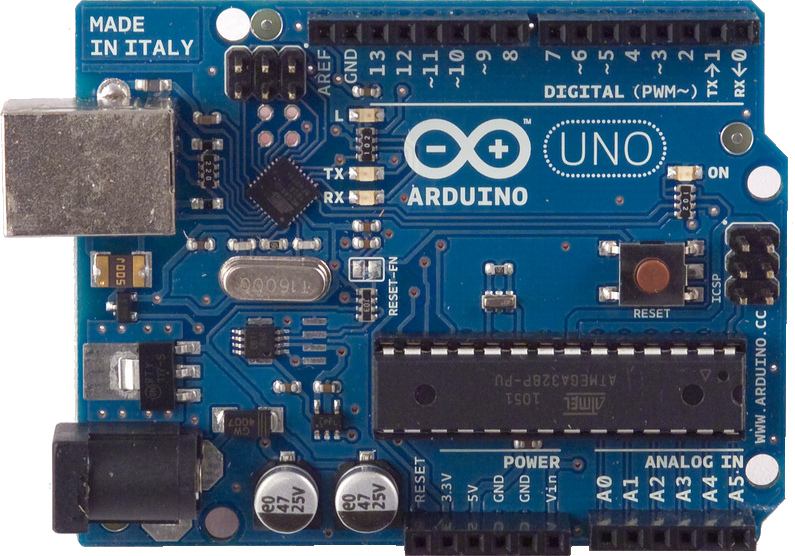
\includegraphics[height=0.33\textheight]{bcollis/1arduino.jpeg}
 
\secrel{1.1 Your learning in Technology
\\\ru{Ваше обучение по специальности <<Технология>>}}

\secdown
\secrel{Technology Achievement Objectives from the NZ Curriculum
\\\ru{Цели обучения технологиям Ново-Зеландской программы}}

\begin{itemize}
  \item \textbf{Technological Practice\\\ru{Технологическая практика}}
  \begin{itemize}
    \item \textbf{Brief}: develop clear specifications for your technology
    projects.\\\ru{\textbf{Чоткость}: разработка ясных описаний для ваших
    технологических проектов.}
    \item \textbf{Planning}: thinking about things before you start making them
    and using drawings such as flowcharts, circuit diagrams, pcb layouts,
    statecharts and sketchup plans while working.\\\ru{\textbf{Планирование}:
    думать прежде чем делать, и использовать во время работы документацию:
    блок-схемы, принципиальные схемы, чертежи разводки плат, диаграммы и
    эскизы.}
    \item \textbf{Outcome Development}: trialling, testing and building
    electronic circuits, designing and making PCBs, writing programs for
    microcontrollers.\\\ru{\textbf{Наработка навыков}: сборка, отладка и
    тестирование электронных схем, проектирование и изготовление печатных плат,
    написание программ для микроконтроллеров.}
  \end{itemize}
  \item \textbf{Technological Knowledge\\\ru{Технологические знания}}
  \begin{itemize}
    \item \textbf{Technological Modelling}: before building an electronic
    device, it is important to find out how well it works first by modelling
    and/or trialling its hardware and software.\\\ru{\textbf{Моделирование}:
    прежде чем строить готовое электронное устройство, сначала важно понять как
    оно работает путем моделирования и/или макетирования аппаратного и
    программного обеспечения.}
    \item \textbf{Technological Products}: getting to know about components and
    their characteristics.\\\ru{\textbf{Технологические продукты}: знания о
    компонентах и их характеристиках.}
    \item \textbf{Technological Systems}: an electronic device is more than a
    collection of components it is a functioning system with inputs, outputs and
    a controlling process.\\\ru{\textbf{Технологические системы}: электронное
    устройство является более, чем набором компонентов, это функционирующая
    система с входами, выходами и контролирующим процессом.}
  \end{itemize}
  \item \textbf{Nature of Technology\\\ru{Природа технологии}}
  \begin{itemize}
    \item \textbf{Characteristics of Technological Outcomes}: knowing about
    electronic components especially micro\-con\-trol\-lers as the basis for
    modern technologies.\\\ru{\textbf{Значение технологических достижений}:
    знания об электронных компонентах, особенно микроконтроллерах, как основе
    современных технологий.}
    \item \textbf{Characteristics of Technology}: electronic devices now play a
    central role in the infrastructure of our modern society; are we their
    masters, how have they changed our lives?\\\ru{\textbf{Роль технологии в
    обществе}: электронные устройства в настоящее время играют центральную роль
    в инфраструктуре нашего современного общества; подчинили ли они нас себе,
    как они изменили нашу жизнь?}
  \end{itemize}
\end{itemize}

\secup

\secrel{1.2 Key Competencies from The NZ Curriculum
\\\ru{Ключевые компетенции Ново-Зеландской программы}}

\begin{itemize}
  \item 
\textbf{Thinking}: to me the subject of technology is all about thinking. My
goal is to have students understand the technologies embedded within electronic
devices. To achieve this students must actively enage with their work at the
earliest stage so that they can construct their own understandings and go on to
become good problem solvers. In the beginning of their learning in electronics
this requires students to make sense of the instructions they have been given
and search for clarity when they do not understand them. 
\\\ru{\textbf{Знания}: для меня предметом технологии является все что относится
к знанию. Моя цель: заставить студентов понимать технологии, заложенные в
электронные устройства. Для достижения этого понимания студенты должны активно
учиться\note{в оригинале \textbf{enage}, англо-калька с \emph{себуанского}, NZ}\
в работе на самом раннем этапе, чтобы они могли построить собственное понимание
предмета и пойти дальше, чтобы стать хорошими решалами проблем. В начале
обучения электронике это требует от студентов восприимчивости к инструкциям,
которые им дают, и поиск ясности, когда они не понимают их.}

After that there are many new and different pieces of knowledge introduced in
class and students are given problem solving exercises to help them think
logically. The copying of someone elses answer is flawed but working together is
encouraged. At the core of learning isbuilding correct conceptual models and to
have things in the context of the ‘big picture’.
\\\ru{Для этого на занятиях рассматриваются много новых и различных элементов
знаний, и студентам выдаются задания на решение проблем, чтобы помочь им мыслить
логически. Копирование чужого ответа наказывается, но приветствуется совместная
работа. В основе обучения лежит построение правильных концептуальных моделей и
анализ в контексте "большой картины".}
  \item 
\textbf{Relating to others}: working together in pairs and groups is as
essential in the classroom as it is in any other situation in life; we all have
to share and negotiate resources and equipment with others; it is essential
therefore to actively communicate with each other and assist one other.
\\\ru{\textbf{Взаимодействие}: работа в парах и группах, это важно как в классе,
так и в любой другой ситуации в жизни; мы все должны договариваться и разделять
ресурсы и оборудование с другими людьми; поэтому крайне важно активное общение и
помощь друг другу.}
  \item 
\textbf{Using language symbols and texts}: At the heart of our subject is the
language we use for communicating electronic circuits, concepts, algorithms and
computer programming syntax; so the ability to recognise and using symbols and
diagrams correctly for the work we do is vital.
\\\ru{\textbf{Использование языка символов и текстов}: сердцем нашего предмета
является язык, который мы используем для обмена информацией в электронных
схемах, планах, алгоритмах и синтаксисе компьютерных языков программирования;
так что способность распознавать и правильно использовать символы и диаграммы
для работы, которую мы делаем, имеет критическое значение.}
  \item 
\textbf{Managing self}: This is about students taking personal responsibility
for their own learning; it is about challenging students who expect to read
answers in a book or have a teacher tell them what to do. It means that students
need to engage with the material in front of them. 
\\\ru{\textbf{Самоконтроль}: студенты принимают на себя личную ответственность
за собственное обучение; они принимают вызов, надеясь найти ответы в книгах или
найти учителя, способного объяснить им, что делать. Это значит, что студенты
должны взаимодействовать с рабочим материалом.}
 
Sometimes the answers will come easily, sometimes they will not; often our
subject involves a lot of trial and error (mostly error). Students should know
that it is in the tough times that the most is learnt. And not to give up keep
searching for understanding.
\\\ru{Иногда ответы приходят легко, иногда нет; часто наша тема требует много
проб и ошибок (в основном ошибок). Студенты должны знать, что у них будут
трудные времена, пока не будет изучена б\'{о}льшая часть. И не сдаться в поиске
понимания.}
  \item 
\textbf{Participating and contributing}: We live in a world that is incredibly
dependent upon technology especially electronics, students need to develop an
awareness of the importance of this area of human creativity to our daily lives
and to recognise that our projects have a social function as well as a technical
one.
\\\ru{\textbf{Участие и содействие}: мы живем в мире, который невероятно зависит
от технологии, особенно электроники; студенты должны развивать осознание
важности этой области человеческого творчества в нашей повседневной жизни, и
понимать, что наши проекты имеют и социальную функцию, а не только техническую.}
\end{itemize}

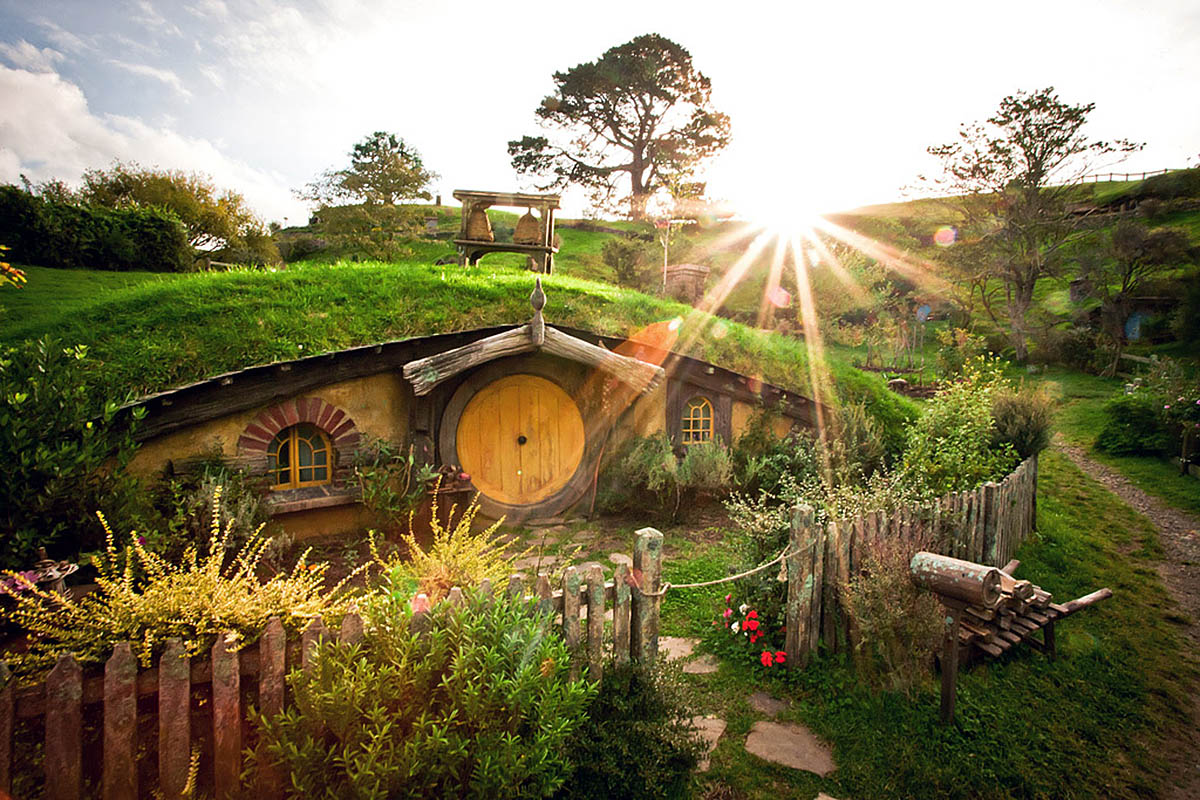
\includegraphics[width=0.8\textheight]{bcollis/12Hobbiton.jpeg}

\secup
